%
% File acl2012.tex
%
% Contact: Maggie Li (cswjli@comp.polyu.edu.hk), Michael White (mwhite@ling.osu.edu)
%%
%% Based on the style files for ACL2008 by Joakim Nivre and Noah Smith
%% and that of ACL2010 by Jing-Shin Chang and Philipp Koehn

\documentclass[11pt,a4paper]{article}
\usepackage[hyperref]{naaclhlt2018}
\usepackage{times}
\usepackage{latexsym}
\usepackage{amsmath}
\usepackage{multirow}
\usepackage{xcolor}
\usepackage{tikz-dependency}
\usepackage{url}
\usepackage{multirow}
\usepackage{graphicx}
\usepackage{subcaption}
\usepackage{arydshln}
\newcommand\BibTeX{B{\sc ib}\TeX}
\DeclareMathOperator*{\argmin}{argmin}
%\def\aclpaperid{214}
\aclfinalcopy
%%%%%%%
\usepackage{graphicx}
\newcommand{\heart}{\ensuremath\heartsuit}

\newcommand{\yjcomment}[1]{\textcolor{orange}{[$_\mathrm{L}^\mathrm{Y}$#1]}}
\newcommand{\nascomment}[1]{\textcolor{blue}{[#1 ---\textsc{nas}]}}
\newcommand{\yicomment}[1]{\textcolor{gray}{[#1 ---\textsc{yi}]}}
\newcommand{\nss}[1]{\textcolor{magenta}{[$_\mathrm{S}^\mathrm{NS}$#1]}}

\title{Parsing Tweets into Universal Dependencies}

\author{Yijia Liu \\
  Harbin Institute of Technology \\
  {\tt yjliu@ir.hit.edu.cn} \\\And
  Yi Zhu \\
  University of Cambridge \\
  {\tt yz568@cam.ac.uk} \\\AND
  Wanxiang Che \quad Bing Qin\\
  Harbin Institute of Technology\\\And
  Nathan Schneider \\
  Georgetown University \\\And
  Noah A. Smith \\
  University of Washington
  }

\date{}

\begin{document}
\maketitle
\begin{abstract}
We study the problem of analyzing tweets with
Universal Dependencies \citep[UD;][]{NIVRE16.348}. We extend the UD guidelines to cover
special constructions in tweets that affect tokenization,
part-of-speech tagging, and labeled dependencies. Using the extended guidelines, we create
a new tweet treebank ({\sc Tweebank v2}) that is four times larger than the (unlabeled) {\sc Tweebank
  v1} introduced by \citet{kong-EtAl:2014:EMNLP2014}. 
We characterize the disagreements between our annotators
and show that it is challenging to deliver
consistent annotation due to ambiguity in
understanding and explaining tweets. Nonetheless, using the new treebank,
we build a pipeline system to parse raw tweets into UD. To overcome 
annotation noise without sacrificing computational efficiency, we propose a new
method to distill an ensemble of 20 transition-based parsers into a single one. Our
parser achieves an improvement of 2.6 in LAS over the un-ensembled baseline 
and outperforms parsers that are state-of-the-art on other treebanks in both accuracy and speed.
\end{abstract}

\section{Introduction}
NLP for social media messages is challenging, because domain
adaptation is required, and also because creating annotated datasets
(e.g., treebanks)
for training and evaluation is hard. 
Pioneering work by \citet{AAAIW113912} 
annotated 7,630 tokens' worth of tweets according to the
phrase-structure conventions of the Penn Treebank
\citep[PTB;][]{Marcus93buildinga}, enabling conversion to Stanford Dependencies.
\citet{kong-EtAl:2014:EMNLP2014} further studied the challenges in
annotating tweets and presented a tweet treebank ({\sc Tweebank}),
consisting of 12,149 tokens and largely following conventions
suggested by \citet{schneider-EtAl:2013:LAW7-ID}, fairly close to 
\citet{Yamada03statisticaldependency} dependencies (without labels). 
Both annotation efforts were highly influenced by the PTB, whose guidelines
have good grammatical coverage on newswire. However, when it comes
to informal, unedited, user-generated text, the guidelines may leave
many annotation decisions unspecified.
%Motivation notes:  explain why UD is attractive (and more attractive
%than what previous work used, which was based on YM).  one reason is
%that it might allow sharing of texts annotated in different genres (or
%even languages, cite Waleed).  but universal annotation schemes are
%challenging!  this paper contends with the challenges of
%applying UD to social media texts.

%In this paper, we propose to parse the tweets in the convention of
%universal dependencies and built up the whole pipeline to parse the
%tweets from the raw text form.

Universal Dependencies \citep[UD]{NIVRE16.348} were introduced to enable
consistent annotation across different languages. To allow such
consistency, UD was designed to be adaptable to different genres \cite{wang-EtAl:2017:Long6} 
and languages \cite{guo-EtAl:2015:ACL-IJCNLP2,TACL892}. We propose that analyzing
the syntax of tweets can benefit from such adaptability. In this paper,
we introduce a new English tweet treebank of 55,607 tokens that follows the UD
guidelines, but also contends with social media-specific challenges that were not
covered by UD guidelines.\footnote{We developed our treebank independently of a similar effort for Italian tweets \cite{sanguinetti-17}. 
See \S\ref{sec:postwita} for a comparison.} Our annotation includes 
tokenization, part-of-speech (POS) tags, and (labeled) Universal Dependencies.
We characterize the disagreements among our annotators and find that
consistent annotation is still challenging to deliver even with
the extended guidelines.

%\nascomment{Points that were in older text that I want to keep around:}
%\begin{itemize}
%\item Despite the informal nature of tweets, we argue that they basically follow the same grammar as their formal language counterpart.
%\item UD was designed to handle the variant syntactic phenomenons across different languages and we expect its `context head' principle will bring convenience to the parsing of informal and even ungrammatical tweets. 
%\yjcomment{I still feel we should give a reason why we choose UD. One
%  example is that twitter users tend to leave out the copula verb and
%  it will be messy for the `function head' principle to deal with this
%  case. One observation is that informal tokens/syntax happens more on
%  function words rather than content word.} \nascomment{maybe we could
%  argue that, if UD is designed to work for many languages, it should
%  also be able to work for dialects, including AAVE, and informal
%  registers.  YM was not designed for cross-linguistic applicability.}
%\end{itemize}

Based on these annotations, we nonetheless designed a pipeline to parse 
raw tweets into Universal Dependencies. Our pipeline includes: a
bidirectional LSTM (bi-LSTM) tokenizer, a word cluster-enhanced POS
tagger \citep[following][]{owoputi-EtAl:2013:NAACL-HLT}, and a stack LSTM parser
with character-based word representations
\cite{ballesteros-dyer-smith:2015:EMNLP}, which we refer to as our
``baseline'' parser.
To overcome the noise in our annotated data and achieve better performance
without sacrificing computational efficiency, we 
distill a 20-parser ensemble into a single greedy  parser 
\cite{DBLP:journals/corr/HintonVD15}.
We show further  that learning directly from the exploration of the ensemble parser
is more beneficial than learning from the gold standard ``oracle''
transition sequence. Experimental results show that an improvement of more
than 2.6 points in LAS over the
baseline parser can be achieved with our distillation method.  It outperforms
other state-of-the-art parsers in both accuracy and speed.

The contributions of this paper include:
\begin{itemize}
\item We study the challenges of annotating tweets in UD (\S\ref{sec:anno})
and create a new tweet treebank ({\sc Tweebank v2}), which includes 
tokenization, part-of-speech tagging, and labeled Universal Dependencies.
We also characterize the difficulties of creating such annotation.

\item We introduce and evaluate a pipeline system to parse the raw tweet text into
Universal Dependencies (\S\ref{sec:parsing}).  Experimental results show
that it performs better than a pipeline of the state-of-the-art alternatives.

\item We propose a new distillation
method for training a greedy parser, leading to better performance
than existing methods and without efficiency sacrifices.
\end{itemize}

We release our dataset and our system as open-source software at
\url{http://anonymized}. 


\section{Annotation}\label{sec:anno}
%\yicomment{Maybe we should contrast UD and kong's annotation strategy during each stage, because UD has also annotation guideline for every stage.}

We first review {\sc Tweebank v1} of \citet{kong-EtAl:2014:EMNLP2014},
the previous largest Twitter dependency annotation effort 
(\S\ref{sec:tweebank}).
Then we introduce the differences in our tokenization
(\S\ref{sec:tok-anno}) and part-of-speech (\S\ref{sec:pos-anno}) (re)annotation with \citet{ICWSM101540} and 
\citet{gimpel-EtAl:2011:ACL-HLT2011}, respectively, on which {\sc Tweebank v1} was built. 
We describe our effort of adapting the
UD conventions to cover tweet-specific constructions (\S\ref{sec:ud-tweet}). 
Finally, we present our process of creating a new tweet treebank, {\sc
  Tweebank v2}, and characterize
the difficulties in reaching consistent annotations (\S\ref{sec:anno-process}).

\subsection{Background: \textsc{Tweebank}}\label{sec:tweebank}

The annotation effort we describe stands in contrast to the previous work
by \newcite{kong-EtAl:2014:EMNLP2014}.  Their aim was the rapid
development of a dependency parser for tweets, and to that end they
contributed a new annotated corpus, \textsc{Tweebank}, consisting of
12,149 tokens.  Their annotations added unlabeled dependencies to a portion of the data
annotated with POS tags by 
\newcite{gimpel-EtAl:2011:ACL-HLT2011} and
\newcite{owoputi-EtAl:2013:NAACL-HLT} after rule-based tokenization \citep{ICWSM101540}.
Kong et al.~also contributed a system for parsing;
we defer the discussion of their parser to \S\ref{sec:parsing}.

Kong et al.'s rapid, small-scale annotation effort was heavily constrained.  It was
carried out by annotators with only cursory training, no clear
annotation guidelines, and no effort to achieve consensus on controversial
cases. Annotators were allowed to underspecify their analyses.
Most of the work was done in a very short amount of
time (a day).  Driven both by the style of the text they sought to annotate
and by exigency, some of their annotation conventions included:
\begin{itemize}
\item Allowing an annotator to exclude tokens from the dependency
  tree.  A clear criterion for exclusion was not given, but many
  tokens were excluded because they were deemed ``non-syntactic.''% \yicomment{including some Twitter specific tokens, which we will refine the definition in Section 2.3 and 2.4?}
\item Allowing an annotator to merge a multiword expression into a
  single node in the dependency tree, with no internal structure.
  Annotators were allowed to take the same step with noun phrases.
\item Allowing multiple roots, since a single tweet might contain more
  than one sentence.
\end{itemize}
These conventions were justified on the grounds of making the
annotation easier for non-experts, but they must be revisited in our
effort to apply UD to tweets.

\subsection{Tokenization}\label{sec:tok-anno}
Our tokenization strategy lies between the strategy of
\citet{ICWSM101540} and that of UD.
There is a tradeoff between preservation of original tweet content and respecting
the UD guidelines.

The regex-based tokenizer of \citet{ICWSM101540}---which was 
originally designed for an exploratory search interface called
TweetMotif, not for NLP---preserves most whitespace-delimited tokens, including 
hashtags, at-mentions, emoticons, and unicode glyphs. 
They also treat contractions and acronyms as whole tokens and do not split them.
UD
tokenization,\footnote{\url{http://universaldependencies.org/u/overview/tokenization.html}}
in order to better serve dependency annotation, treats each syntactic word as a token.
They therefore more aggressively split
clitics from contractions (e.g., {\it  gonna} is tokenized as {\it gon} and {\it na}; {\it its}
is tokenized as {\it it} and {\it s} when {\it s} is a copula).
%\yicomment{are words like gonna called contractions, or do they have
%another term?}. \nascomment{yes}
But acronyms are not touched
in the UD tokenization guidelines. Thus, we follow the UD tokenization for contractions
and leave acronyms like {\em idc} (``I don't care'') as a single token. 
%\nascomment{unless we make a change, I think we need to say
%  here that acronyms like \emph{idc} are left as a single token}
%\yjcomment{mentioned acronymns, we don't have the problem of normalization, cause
% normalization was just annotated for data study.}

In the different direction of splitting tokens, UD guidelines also suggest to merge
{\it multi-token words} (e.g., {\it 20 000}) into one single token in some special
cases. We witnessed a small number of tweets that contain multi-token words
(e.g., {\it Y O}, and {\it R E T W E E T}) but didn't combine them for simplification.
Such tokens only account for 0.07\% and we use the UD
  {\it goeswith} relation to resolve these cases in the dependency annotations.

\subsection{Part-of-Speech Annotation}\label{sec:pos-anno}

Before turning to UD annotations, we (re)annotated the data with 
POS tags, for consistency with other UD efforts,
which adopt the universal POS tagset.\footnote{A revised and extended version of \citet{PETROV12.274} with 17 tags.}
% The POS annotation of a word in tweets is generally based on its syntactic distribution, which indicates that the POS of word changes on different context.
% Sticking to the syntactic distribution makes it possible that a `$\heart$' symbol is tagged as a verb as shown in Figure \ref{fig:non-syn-toks}. \yjcomment{Need a better explanation.}
%We follow the UD V2 morphology guideline and use the Universal POS tags~ to tag the tweet tokens. For twitter specific linguistic phenomena, we have set different strategies and try to align with the UD conventions and UD\textunderscore English as close as possible.\footnote{\url{https://github.com/UniversalDependencies/UD\_English}}
In some cases,  non-corresponding tag conflicts arose between the UD English 
treebank conventions \cite[UD\_English;][]{Marneffe2014UniversalSD}\footnote{\url{https://github.com/UniversalDependencies/UD_English}}
and the conventions of \newcite{gimpel-EtAl:2011:ACL-HLT2011}.  %\yicomment{The conflicts
                                %should refer to a {\bf
                                %noncorresponding tag} from that of
                                %gimpel to UDEnglish, cuz they dont
                                %have the same tagset.} 
In these cases, we always
conformed to UD, enabling consistency (e.g., when we exploit the
existing UD\_English treebank in our parser for tweets, \S\ref{sec:parsing}).  For example,  
the nominal URL in Figure \ref{fig:informal-toks} is tagged as {\it
  other} ({\tt X}) and {\tt +} is tagged as {\it symbol} ({\tt SYM})
rather than {\it conjunction} ({\tt CCONJ}).  
% Such violation is resulted by our attempt of conforming the annotation to the {\it universal dependencies - English dependency treebank} (UD\_English), in which all the URLs are tagged as {\it other} and symbolic conjunctors are tagged as {\it symbol}.
% By conforming our annotation to the UD\_English data, hopefully, the tools we built on tweets can benefit from the dataset on broader domain. \yjcomment{need wording}

Tokens that do not have a syntactic function (see Figure \ref{fig:non-syn-toks}, discussed at greater
length in the next section) were usually annotated as \emph{other}
(\texttt{X}), except for emoticons, which are tagged as \emph{symbol}
(\texttt{SYM}), following UD\_English.

% Again, there are un-conventional linguistic constructions in tweets that syntactic distribution doesn't handle well.
% One of the cases is the non-syntactic tokens.
% We consider most of them as {\tt X}, except for the sentiment emoticons, which would be tagged as {\tt SYM}, in practice of matching the UD\_English.
% Another case is the retweet construction which is considered as a non-syntactic phrase and both the RT and at-mention are tagged as {\tt X}.
% For the at-mention, we tag them as proper noun ({\tt PROPN}) in spirit of following the vocative example in UD\_English.
%In token level phenomena, for non-syntactic tokens,  
%For syntactic tokens, we tag them considering their corresponding syntactic function.

%In structure level phenomena, we think {\tt RT @user} in retweet structure have no contribution to the tweet syntax and tag both of them as X.
%We tag usernames in at-mentioned structure as PROPN as they present the vocative case.

Tokens that abbreviate multiple words, such as \emph{idc} are resolved to the POS of the syntactic head of the
expression, following UD conventions (in this example, the head \emph{care} is
a verb, so \emph{idc} is tagged as a verb).
% The informal syntactic tokens can generally be handled by their distribution.
% However, one of the exception is the {\tt phrasal abbreviations} in which one token carries multiple syntactic functions.
% In dealing with such phrases, we propose a routine that first recover their original forms, then, use the POS of their syntactic head word as the POS of the whole phrase.
% Therefore, {\it idc} (I don't care) is a verb because {\it care} is its syntactic head.
% Such routine works for most of the phrasal abbreviations.
When the token is not phrasal, we use the POS of the left-most
sub-phrase.  For example, \emph{mfw} (``my face when'') is tagged as a
noun (for \emph{face}).  % \footnote{Such failure can be resulted by the mis-match of phrase boundaries between the original form and the definition of `phrase' in UD. For example, `mfw' (my face when) doesn't make a phrase because `when' belongs to the subordination that modifies `my face'.}

%In Fig.~\ref{ex1}, {\tt RT} {\tt @yijialiu}, {\tt \#ACL2017}, {\tt http://url} and {\tt th} are all tagged as X and {\tt :)} is tagged as SYM. 
%{\tt rn} is tagged as ADV.
%We should note that multiple tokens are actually included in a phrasal abbreviation, and we use one of their tags as the tag of the whole abbreviation according to their dependency relation or semantic priority.
%aIf there is a hierarchy in the abbreviation, we use the tag of the head word. In UD, ``Right'' is the dependent of ``now '' in the dependency of {\tt rn}, so we tag {\tt rn} as ADV. 
%Although there is no head word in {\tt im}, we think that the subject is usually more informative than the tense in many downstream tasks such as semantic role labelling, so we use the tag of ``I'', e.g. PROPN as the tag of {\tt im}.  
%In Fig.~\ref{ex2}, {\tt RT} and {\tt $\heart$} would be tagged as VERB, {\tt http://url} as X, {\tt \#Awesome} as ADJ, {\tt \#NAACL}, {\tt @zypandora} and {\tt @nlpnoah} as PROPN. One exception is that we tag URLs always as X regardless whether they are syntactic tokens. The reason is that we observed, in UD\_English, that the URLs are all tagged as X and we want to conform with the UD dataset, although we think it is not appropriate and should be changed to tags such as PROPN when they are treated as syntactic tokens.

Compared to the effort of
\newcite{gimpel-EtAl:2011:ACL-HLT2011}, our approach simplifies some
matters.  For example, if a token is not considered syntactic by UD
conventions, it gets an \emph{other} (\texttt{X}) tag (Gimpel et
al.~had more extensive conventions).  Other phenomena, like
abbreviations, are more complicated for us, as discussed above;
Gimpel et al.~used a single part of speech for such expressions.

%  proposed a course grain twitter POS tagset that handles most of the token level phenomena.
% However, our work diverge theirs in several ways.
% Compared with the Gimpel's work, which assigns different tags to non-syntactic tokens in different categories, we simplify them into the {\tt X} tag.
% At the same time, all the abbreviations in \newcite{gimpel-EtAl:2011:ACL-HLT2011} are tagged with one POS, which doesn't distinguish their syntactic functions.
% We argue that such approach over-simplify the abbreviations.
% One example is that {\it idc} (I don't care) and {\it rn} (right now) carries significantly different syntactic functions and should not be treated as the same.
% In this paper, we stick more to the syntactic distribution when handling such abbreviations and it allows them to function differently in different context.

Another important difference follows from the difference in
tokenization.  As discussed in \S\ref{sec:tok-anno}, UD calls for more
aggressive tokenization than that of \citet{ICWSM101540} which opted
out of splitting contractions and possessives. As a consequence of adopting \citet{ICWSM101540}'s tokenization, 
Gimpel et al.~introduced new parts of speech for these cases
instead.\footnote{These tags only account for 2.7\% of tokens,
  leading to concerns about data sparseness in tagging and all
  downstream analyses.}  For us, these tokens must be split, but
universal parts of speech can be applied.

%  is resulted by the tokenization process.
% In \newcite{gimpel-EtAl:2011:ACL-HLT2011}, they opted out the tokenization on contractions and possessives and introduce several tags for these un-tokenized words.
% As mentioned above, the goal of conforming our annotation to the UD\_English makes us adopt the same the UD-styled tokenization.
% Thus, these tags for contractions and possessives are not necessary at all in our case.
% What's more, as \newcite{gimpel-EtAl:2011:ACL-HLT2011} mentioned, only a small proportion of tokens can be categorized into these tags (2.7 \% in total), which casts a doubt of the usefulness of these tags.
% %However, we found that their methods did not conform with UD conventions and our strategies have some advantages over their tagset. We discuss the main difference as follows.
% %The first difference lies in the tokenizations.
% %\newcite{Gimpel:2011:PTT:2002736.2002747} opted not to split contractions or possessives and introduced four new tags (S, Z, L, M) for combined forms: \{nominal, proper noun\} $\times$ \{verb, possessive\}. 
% %Major concern of designing such tags is to minimize the effort of tokenization, but it is not comprehensive and far from including all of the possible combinations of POS tags within the contractions. 
% %What's more, only a small proportion of tokens can be categorized into these tags (2.7 \% in total), which casts a doubt of the usefulness of these tags.
% %Instead UD conventions suggest that we put such complexity into the tokenization module and split contractions and possessives, then tag them accordingly, so that we do not need extra POS tags for the combined forms.
% %The second difference is that although the phrasal abbreviations are not split in both methods, they use tag G for all the phrasal abbreviations, while we use the tag of the head word or the highest hierarchical word in terms of dependencies as the tag of the whole phrasal abbreviations. 
% %We think it is not reasonable to treat the phrasal abbreviations in the same part of speech because obviously abbreviations can have different syntactic functions and we want to preserve the most useful information for both parser and the downstream tasks. For example, {\tt wtf} could be tagged as PRON or INTJ according to the context, and {\tt rn} is usually tagged as ADV. Tagging them merely as G will definitely lose much information.
% %Third, special tags were designed to handle twitter or online special tokens such as URLs, hashtags and emoticon in \newcite{Gimpel:2011:PTT:2002736.2002747}. However, in most cases, as long as theses tokens are non syntactic, they play the same role in tweets, hence should be tagged the same. In this paper, except for the emoticon and emoji, tagged as SYM, we tag all the other non-syntactic tokens as X.


\subsection{Universal Dependencies Applied to Tweets} \label{sec:ud-tweet}

We adopt UD version 2 guidelines to annotate the syntax of tweets.
In applying UD annotation conventions to tweets, the choices of 
\newcite{kong-EtAl:2014:EMNLP2014} must be revisited.  We consider the
key questions that arose in our annotation effort, and how we resolved them.

% Linguistic phenomena
	% word level
		% RT
		% Hashtag
		% Mention, urls
		% Symbols and Emoticons
		% Truncated tokens
	% twitter level
		% RT
		% Parataxis	
% POS
	% Acronym priority
	% URL tagged as X	
% Depenency
	% Concentrate on NON-UD phenomena
% Statistics
	% Scale
	% Inter-annotator agreement
	% Proportion
		% how many hashtags, mentions, ....
		% how many acornyms

%\subsection{Linguistic Phenomena of Twitter} \label{lingphen}
% Twitter, as an extreme example of informal domain, contains a collection of conversational languages (like abbreviation, informal contraction, and variant entity names) and twitter-specified markers (like retweet mark, and username).
% The key issue lies in understanding the specific construction that doesn't carry any syntactic functions, and designed rules to handle the specific constructions in tweets.
% In the following section, we studied such constructions from both the token and structure level. \yjcomment{I don't like the name of \textbf{structure level}}
% %As the representative of the web language, different from the standard languages such as newswire, twitter has its own linguistic phenomena, that could be categorized into token level and structure level phenomena, and we will discuss them separately.


\paragraph{Acronym abbreviations.}  % How should we syntactically
% analyze acronym tokens like \emph{idc}
% (abbreviating ``I don't care'')
%  and \emph{rn} (``right now'')?  Should
% they be decomposed into their component words, and if so should those
% words be ``normalized'' into explicitly spelled out intermediate
% forms? \yicomment{this sentence should be deleted or moved to tokenization?} \yicomment{As we already know from previous sections, \emph{idc} is not tokenized and tagged as verb, we follow ...} \yicomment{Normalization is discussed in the 2.5.2 Annotation Process. Actually we did do normalization, but just as auxiliary info, didn't use it for any model.}\yjcomment{i think acronym is a different story to tokenization.}
We follow \citet{kong-EtAl:2014:EMNLP2014} and annotate the
syntax of an acronym as a single word without normalization. Their syntactic functions
are decided according to their context. \citet{eisenstein:2013:NAACL-HLT} studied the necessity of normalization
in social media text and argued that such normalization is problematic.
Our solution to the syntax of abbreviations follows the spirit of his argument. Because abbreviations which clearly carry
syntactic functions only constitute 0.06\% of the tokens in our
dataset, we believe that normalization for acronyms is an unnecessarily complicated
step.
% \nascomment{maybe we owe citations to
%   \cite{finin-EtAl:2010:MTURK,eisenstein:2013:NAACL-HLT} here?  maybe
%   better papers to cite}


\paragraph{Non-syntactic tokens.}  
\begin{table}
\centering
\begin{tabular}{lrr}
\hline
\multicolumn{2}{r}{syntactic (\%)} & non-syntactic (\%)\\ \hline
emoticons & 0.25 & 0.95 \\
RT & 0.14 & 2.49\\
hashtag & 1.02 & 1.24 \\
URL & 0.67 & 2.38 \\
truncated words & 0.00 & 0.49 \\
 \hline
 total & 2.08 & 7.55 \\
 \hline
\end{tabular}
\caption{Proportions of non-syntactic tokens in our annotation. %\yicomment{should add also retweet at-mentions}
These statistics are obtained on 140 character-limited tweets. \label{tbl:non-synt-prop}}
\end{table}

\begin{figure*}[t]
	\centering
	\small
	\begin{dependency}[edge slant=2, text only label, label style=above]
		\begin{deptext}
			Perfect \& \textcolor{red}{\bf $\heart$} \& \textcolor{orange}{\bf RT} \& \textcolor{orange}{\bf @coldplay} \& : \& Fix \& You \& from \& the \& back \& \textcolor{gray}{\bf \#ColdplayMinneapolis} \& \textcolor{blue}{\bf http://bit.ly/2dj2WCl} \& Nice \& \textcolor{cyan}{\bf p} \& ...\\
			\tiny ADJ \&\tiny SYM \&\tiny X \&\tiny X \&\tiny PUNCT \&\tiny VERB \&\tiny NOUN \&\tiny ADP \&\tiny DET \&\tiny NOUN \&\tiny X \&\tiny X \& \tiny ADJ \& \tiny X \& \tiny PUNCT \\
		\end{deptext}
		\deproot{1}{root}
		\depedge[edge unit distance=1em]{1}{2}{discourse}
		\deproot{6}{root}
		\depedge[edge unit distance=1em]{6}{3}{discourse}
		\depedge[edge unit distance=1em]{3}{4}{discourse}
		\depedge[edge unit distance=1em]{3}{5}{punct}
		\depedge[edge unit distance=1em]{6}{7}{obj}
		\depedge[edge unit distance=0.8em]{6}{10}{obl}
		\depedge[edge unit distance=1em]{10}{8}{case}
		\depedge[edge unit distance=1em]{10}{9}{det}
		\depedge[edge unit distance=0.8em]{6}{11}{discourse}
		\depedge[edge unit distance=0.8em]{6}{12}{list}
		\deproot{13}{root}		
		\depedge[edge unit distance=0.8em]{13}{14}{discourse}
		\depedge[edge unit distance=0.8em]{13}{15}{punct}
	\end{dependency}
	\caption{An example to illustrate non-syntactic tokens:
		\textcolor{red}{sentiment emoticon},
		\textcolor{orange}{retweet marker and its following at-mention},
		\textcolor{gray}{topical hashtag},
		\textcolor{blue}{referential URL}, and
		\textcolor{cyan}{truncated word}.
		This is a concatenation of three real tweets.
	}\label{fig:non-syn-toks}
\end{figure*}

\begin{figure*}[t]
	\centering
	\small
	\begin{dependency}[edge slant=2, text only label, label style=above]
		\begin{deptext}
			@username \& its \& \#awesome \& u \& gonna \& $\heart$ \& it \& Chk \& out \& our \& cooool \& project \& on \& http://project\_link \& + \& RT \& it\\
			\tiny PROPN \& \tiny PRON \& \tiny ADJ \& \tiny PRON \& \tiny VERB \& \tiny VERB \& \tiny PRON \& \tiny VERB \& \tiny ADP \& \tiny PRON \& \tiny ADJ \& \tiny NOUN \& \tiny ADP \& \tiny X \& \tiny SYM \& \tiny VERB\& \tiny PRON\\
		\end{deptext}
		\deproot{3}{root}
		\depedge[edge unit distance=1em]{3}{1}{vocative}
		\depedge[edge unit distance=1em]{3}{2}{nsubj}
		\depedge[edge unit distance=1em]{3}{5}{parataxis}
		\depedge[edge unit distance=1em]{5}{4}{nsubj}
		\depedge[edge unit distance=1em]{5}{6}{xcomp}
		\depedge[edge unit distance=1em]{6}{7}{obj}
		\depedge[edge unit distance=0.7em]{3}{8}{parataxis}
		\depedge[edge unit distance=1em]{8}{9}{compound:prt}
		\depedge[edge unit distance=0.7em]{8}{12}{obj}
		\depedge[edge unit distance=1em]{12}{10}{nmod:poss}
		\depedge[edge unit distance=1em]{12}{11}{amod}
		\depedge[edge unit distance=0.6em]{8}{14}{obl}
		\depedge[edge unit distance=1em]{14}{13}{case}
		\depedge[edge unit distance=0.55em]{8}{16}{conj}
		\depedge[edge unit distance=1em]{16}{15}{cc}
		\depedge[edge unit distance=1em]{16}{17}{obj}
	\end{dependency}
	\caption{An example to illustrate informal but syntactic tokens.
		This is a contrived example inspired by several tweets.}\label{fig:informal-toks}
\end{figure*}

The major characteristic that distinguishes tweets from standard texts is that
a large proportion of tokens don't carry any syntactic function. 
In our annotation, there are five types of non-syntactic tokens commonly seen in tweets: %\yicomment{need to say it explicitly that here we only refer to Twitter/web specific tokens, not including exclamations or punctuations or other stuffs. Or we can say punctuations and exclamations are canonically non-syntacitc}: 
sentiment emoticons, retweet markers and their following at-mentions, topical hashtags, referential URLs, and
truncated words.\footnote{The tweets we analyze have at most 140
  characters. Although Twitter has doubled the tweet length limit to
  280 characters since our analysis, we believe this type of token
  will still remain.}  Figure \ref{fig:non-syn-toks} illustrates examples of
these non-syntactic tokens.  As discussed above, these are generally
tagged with the \emph{other} (\texttt{X}) part of speech, except
emoticons, which are tagged as \emph{symbol} (\texttt{SYM}).  In our annotation, 
7.55\% of all tokens are belong to one of the five types; detailed statistics can be found in Table \ref{tbl:non-synt-prop}.
%\yjcomment{I've merged retweet marker and retweet at-mention into one.}

It is important to note that these types may, in some
contexts, have syntactic functions.
For example, besides being a discourse marker, \emph{RT} can
abbreviate the verb {\it retweet}, and emoticons and hashtags may be
used as content words within a sentence, and at-mentions can be normal vocative proper nouns; see Figure
\ref{fig:informal-toks}.  Therefore, the criteria for annotating a
token as non-syntactic must be context-dependent.
%To our knowledge, this issue has not previously been addressed in UD
%annotation efforts \nascomment{check!}\yjcomment{it's not safe to claim that.}.


Inspired by the way UD deals with \emph{punctuation} (which is
canonically non-syntactic), we adopt the following
conventions%\yicomment{this applies to all non-syntactic tokens including punctuations and excalamations}
:
%\yicomment{shall we mention how we segment sentences? Seems relevant
%here}\yjcomment{i don't want to touch sentence segmentation, it will
%makes the paper more messy.}\nascomment{agree with Yijia}

\begin{itemize}
%\item For the at-mentions in retweet constructions, we attach them to their retweet markers. We will discuss our choice in the following paragraph;
\item If a non-syntactic token is within a sentence that has a clear predicate, it will be attached to this predicate. Retweet construction is a special case and we will discuss our choice in the following paragraph.
\item If the whole sentence is made of a sequence of non-syntactic tokens, we attach all these tokens to the first one.
%\item In parataxis case, when it is difficult to decide which sentence or phrase x should belong to, we always attach x to the previous predicate of the paratactic clause or phrase;
\item Non-syntactic tokens are mostly labeled as {\it discourse}, but
  URLs are always labeled as {\it list}, following the UD\_English dataset.% \yicomment{need to add punct for punctuations?}
%\\ \yicomment{For retweet at-mention case, we attach the retweet at-mentions to the RT sign, so that the retweet action and the people whose tweet is being retweeted could be connected.\footnote{We can also follow the first convention to attach the retweet at-mention to its predicate, but we think it is better for downstream tasks.}}
\end{itemize}



% \subsubsection{Token Level}
% \paragraph{Informal Syntactic Tokens.}
% Informal tokens like phrase abbreviation (like {\tt mfw}: my face when, {\tt rn}: right now, and etc.) and orthographic variants (like {\tt sooo cooool}) have drawn much attention in previous literals \cite{finin-EtAl:2010:MTURK,eisenstein:2013:NAACL-HLT} \yjcomment{not sure orthographic variants is a good name, need reference.}
% However, in the sense of syntactic functions, they work in the same way as the ordinary words, which makes them requires less specialty in designing annotation conventions.
% %Syntactic tokens are just like normal tokens in the standard text.
% %They always have syntactic functions in tweets.
% %They could be orthographic variants or abbreviations that represents a phrase.

% \paragraph{Non-syntactic Tokens.}

% Besides the informal but syntactic tokens, there are a large collection of tokens that cannot be handled by the syntactic theory designed for standard text.
% A major part of these tokens consists of meta data in tweets, like the sentiment emotion, retweet mark, topical hashtag, and referential URL shown in Figure \ref{fig:non-syn-toks}. 

% However, whether a token convey some syntactic function cannot be simply decided by its form.
% For example, besides being a discourse marker, {\tt RT} can also works as a abbreviation of the verb {\tt retweet}.
% Emoticons are sometimes used as a verbal part of the sentence.
% Twitter users have developed a casual habit of using hashtag, and even use hashtag as a adjective.
% The sentence in Figure \ref{fig:informal-toks} gives a comprehensive example of those informal but syntactic tokens.
% It shows whether a token makes a non-syntactic one is highly conditioned on its context.

% A kind of token that doesn't carry clearly syntactic functions can be resulted by the 140 characters limits of tweets.
% Since last tokens that exceeding 140 characters limits are truncated in tweets which leaves a broken sentence, it is impossible to fully recover their original form and figure out their syntactics.
% In this paper, we propose to treat these truncated tokens, along with the other 4 kinds of tokens mentioned above, as ones without syntactic functions.

\newcite{kong-EtAl:2014:EMNLP2014} proposed an additional
preprocessing step, \emph{token selection}, in their annotation process.
They required the annotators to first select the non-syntactic
tokens and exclude them from the final dependencies annotation.
%  \nascomment{confusing.  were they removed or
%  just labeled as non-syntactic and then excluded from the tree?  I
%  think they were not actually removed, and were still available,
%  e.g., for defining features of the input for parsing}
In order to keep our annotation conventions in line with UD norms and preserve the original tweets as much as possible,
we include non-syntactic tokens in our annotation following the
conventions above. Compared with \citet{kong-EtAl:2014:EMNLP2014},
we also gave a clear %\yicomment{much clearer}
definition of non-syntactic tokens, which helped
us avoid confusion during annotation.

%In the sense of dealing with the non-syntactic tokens, \newcite{kong-EtAl:2014:EMNLP2014} proposed an preprocessing step named {\it token selection} to remove non-syntactic tokens from the original tweets.
%However, concrete standard of non-syntactic tokens was not presented in their work.
%What's more, these unselected tokens are absent from downstream processing, including parsing.
%We differ from their work by proposing concrete standard of non-syntactic tokens and we include these non-syntactic tokens in our final analyzed dependencies by adding special attachment to them.
%There are special tokens that will appear only or much more frequently in tweets.
%According to the syntactic functions these tokens have in the tweets, we classify them into three types: syntactic tokens, non-syntactic tokens and optionally syntactic tokens. 
%Non-syntactic tokens are tokens that will not have syntactic function in tweets, and they are not considered in the syntax analysis and need to be treated independently.
%Optionally syntactic tokens are tokens that can have either syntactic or non-syntactic functions based on the context. Usually they are tokens like URLs ad hashtags that do not participate in the syntax of the tweets, and we treat them as non-syntactic functions by default. However, similar in the analysis of \newcite{Gimpel:2011:PTT:2002736.2002747} and \newcite{kong-EtAl:2014:EMNLP2014}, in some cases they are perceived as the arguments or predicates of tweets and therefore have syntactic functions. In this case we treat them as syntactic tokens.

%Here is a complete list of the special tokens in tweets classified in three types.
%
%\begin{itemize}
%\item syntactic tokens
%	\begin{itemize}
%		\item phrasal abbreviations: {\tt wtf} (what the fuck), {\tt rn} (right now), etc.
%		\item orthographic variants: {\tt u} (you), {\tt sooooo}, {\tt dat} (that), etc.
%	\end{itemize}
%\item Non-syntactic tokens
%	\begin{itemize}
%		\item truncated tokens: last tokens that are truncated in tweets exceeding twitter character limits. Although It might be possible to recover the original tokens from the context in some cases, it is still extremely hard to further predict the rest of the truncated part.
%	\end{itemize}
%\item Optionally syntactic tokens
%	\begin{itemize}
%		\item retweet discourse marker: RT
%		\item URL: http://bit.ly/xyz
%		\item hashtag: \#ACL
%		\item at-mentioned username: @user
%		\item emoticons and emojis: :), :-), $\heart$, etc.
%	\end{itemize}
%\end{itemize}

%As optionally syntactic tokens will be treated as syntactic or non-syntactic tokens based on the specific context, for the sake of simplicity, if not necessary, we will only discuss the syntactic and non-syntactic tokens in the following sections.

\paragraph{Retweet construction.} Figure \ref{fig:non-syn-toks} shows
an example of the retweet construction (\emph{RT @coldplay :}).  This
might be treated as a verb phrase, with \emph{RT} as a verb and the
at-mention as an argument.
% \yicomment{or might be treated as 2 non-syntactic tokens and a punctuation, which should all attach to the predicate of the following retweeted tweet.}
%\yjcomment{i wouldn't like the readers to think in this direction.}.
  This solution would lead to an uninformative root
word and, since this expression is idiomatic to Twitter, might create
unnecessary confusion for downstream applications aiming to identify
the main predicate(s) of a tweet.  We therefore treat the whole
expression as non-syntactic, including assigning the \emph{other}
(\texttt{X}) part of speech to both \emph{RT} and \emph{@coldplay},
attaching the at-mention to \emph{RT} with the \emph{discourse}
label and the colon to \emph{RT} with the \emph{punct}(uation) label,
and attaching \emph{RT} to the predicate of the following sentence.
%\yicomment{since we have introduced retweet at-mentions in the non-syntactic tokens, here we can just briefly justify our choice.}. 

% \nascomment{smooth this in: } Considering the twitter specific constructions, we will treat the retweet construction as a whole non-syntactic phrase, and the inner structure will always be attaching {\tt at-mention} to {\tt RT} with {\tt discourse}, {\tt :} to {\tt RT} with {\tt punct}.
% The whole construction headed on the {\tt RT} marker modifies the predicate of following sentence.
% For the at-mentioned structure, we attach at-mentioned username to the predicate of the most relevant sentence with {\it vocative} label.


\paragraph{Constructions handled by UD.}  A number of constructions
that are especially common in tweets are handled by UD
conventions: ellipsis, irregular word orders, and paratactic phrases
and sentences 
not explicitly delineated by punctuation.
	
% \subsubsection{Structure Level}
% The syntactic constructions vary greatly across different tweets.
% Unconventional constructions which frequently occur include ellipsis, irregular word orders, and para-tactic sentences without the segmentation of punctuations \yjcomment{I move the 3rd bullet point here because this construction was handled by UD-guidelines}.
% And these unconventional ones are more or less resolved by the universal dependencies.
% The unresolved cases are mainly resulted by the format of twitter.
% The {\it retweet} and {\it at-mention} are of two major constructions.
% \paragraph{Retweet.} For the {\it retweet} construction (`{\tt RT @coldplay :}' in Figure \ref{fig:non-syn-toks}), although it can be treated as a verbal phrase in which retweet marker works as a verb and the following at-mention is its objective, we argue that such convention lead to a uninformative root word.
% It also increase the difficulty for downstream tasks in figuring out the core predicate and arguments for one certain tweet.
% Thus, we treat the whole construction as a non-syntactic phrase. \yjcomment{correct me if I am wrong.}

\paragraph{Vocative at-mentions.}  Another idiomatic construction on
Twitter is a vocative at-mention (sometimes a
signal that a tweet is a reply to a tweet by the mentioned user). % \yicomment{not necessary, can be just mentioning somebody. should be careful to say it. We can say this construction include 1. reply;  2. mention sb. Both cases are similar to general vocative proper noun case in standard texts. And we need to exclude at-mentions in Retweet Construction.}\yjcomment{i didn't see any difference between reply and mention, they all starts with a @username.}.
We
treat these at-mentions as vocative expressions, labeling them with
POS tag
\emph{proper noun} (\texttt{PROPN}) and attaching them to the
main predicate of the sentence it is within with the label \emph{vocative} as in UD guidelines (see Figure \ref{fig:informal-toks} for an example).

\subsection{Comparison to PoSTWITA-UD}\label{sec:postwita}
\citet{sanguinetti-17} presented the \textit{PosTWITA-UD} which is
the first Twitter treebank in Universal Dependencies.
In their convention, tokenization tends to preserve the original
tweet content but two special cases, \textit{articulated prepositions}
and \textit{clitic clusters}, are tokenized.
Beyond tokenization, an extra layer of lemmas is annotated
to recover ``what is understandable by a human''.
It's arguable that normalization (the lemmatization in \citet{sanguinetti-17})
on social media data is essential according to \citet{eisenstein:2013:NAACL-HLT}.
In this paper, we don't include normalization and leave it an open question for further study.

In the syntax annotation, tweet specific
constructions are considered by both \citet{sanguinetti-17} and our paper.
We agree on the syntax head in these constructions but differ on
the choice of relations for depicting these constructions.
We use \textit{discourse} for topical hashtag and \citet{sanguinetti-17} used \textit{parataxis}. 
Similar difference happens in referential URLs where we use \textit{list} by following UD\_English and they use \textit{dep}.
The choice of relation on the non-syntactic tokens is questionable
since UD doesn't have specified guideline for this. 
Our choice of \textit{discourse} is inspired by the observation that emoticon is annotated as \textit{discourse}. Non-syntactic tokens can be easily recovered
from our annotation and changing it to other relation in the future development is not difficult.

%Ho \textit{non-syntactic tokens} (like sentiment emoticon, topical hashtag).

\nss{discuss similarities and differences of conventions to \cite{sanguinetti-17}. 
We expect that the official UD guidelines will eventually adopt standards for these issues so the treebanks can be harmonized.}
\yjcomment{i've finished this part.}

% \paragraph{At-mention.} At-mention in the beginning of a tweet is the format of indicating the `reply' action.
% In this paper, we treat the at-mentions as vocative expressions for their connections with the traditional vocative words, rather than treat them as non-syntactic metadata, which increase the complexity for analyzing a tweet.
% \yjcomment{since the original discussion mainly focus on tokens, I move them to the former section.}
% %Besides the token level phenomena of twitter, there are also structural patterns appearing in the twitter.

%\begin{itemize}
%\item Retweet structure: {\tt RT @user : \{tweet content\}} is a typical structural pattern when a user is retweeting from other users. 
%\item At-mentioned structure: Except the retweet structure and syntactically at-mentioned username, we think that all of other at-mentions are vocative case, usually appearing at the beginning or the end of the sentences in tweets.
%\item Paratactic parts without punctuations: We use ``part'' to refer to a self-contained clause or phrase, which is independent of other ``part''. Very often, one tweet is comprised of multiple parts without any delimiting punctuations, such as {\tt \{part 1\} \{part 2\} ...}
%\end{itemize}

%We treat retweet structure and at-mentioned structure as structural patterns and keep their annotations consistent across tweets. For parataxis case, we treat each single sentence or phrase normally, and connect them together following the UD conventions. 

%From Fig.~\ref{ex1}, we argue that {\tt u} and {\tt rn} are syntactic tokens.
%{\tt th} is a truncated token and does not have any syntactic function, although we can infer that the {\tt th} could be probably {\tt the}.
%{\tt \#ACL2017}, {\tt :)} and {\tt http://url} are optionally syntactic tokens, and should be all treated as non-syntactic tokens in this example.
%{\tt RT @Yijia :} should be analyzed as the retweet structure, and {\tt heading to Canada for ACL} and {\tt can u gimme some money} should be considered as paratactic clauses without punctuations.
%
%However, consider another example in Figure \ref{fig:informal-toks}. All of the optionally syntactic tokens ({\tt RT}, {\tt http://url}, {\tt \#NAACL}, {\tt \#Awesome}, {\tt @zypandora}, {\tt @nlpnoah} and {\tt $\heart$}) have syntactic functions, and we need to take them into account in the syntactic analysis.

% \subsection{Dependency Annotation}

%We follow the UD v2 syntax guideline and the English specific {\it universal dependency relations} to annotate our data.

%In token level phenomena, we adopt the following rules for non-syntactic tokens, denoted as x: 
%Again, as shown in Section \ref{sec:pos-anno}, the major challenge in adopting UD on tweets lies on dealing with the non-syntactic parts.

%If it is hard to decide which sentence would be the most relevant, we attach it to the previous sentence's predicate.
	%\item Paratactic parts without punctuations: we follow the UD convention, set the first part as the main part of the sentence, and set its predicate as the main predicate of the sentence. Every predicate of the following parts should attach to the main predicate. If the main part and some following part are both phrases, the label is {\it list}, otherwise the label is {\it parataxis}. Note that we still have an exception for URLs, conforming with UD, which are always labelled as {\it list}, regardless of the type of the other part.
%\end{itemize}

% Besides these non-syntactic and special constructions, the informal but syntactic tokens are treated in the same way with their original form.

%We further adopt the following rules for structure level phenomena:


% unlabelled, Informal
% exclude non-syntactic tokens, punctuations
% Annotation conventions
%\newcite{kong-EtAl:2014:EMNLP2014} presented a syntactic treebank on Gimpel et al.'s POS tagset.
%Compared with their work which create an unlabeled treebank, we further attach dependency relations and it's expected to be more helpful for the downstream tasks.
%We also provide concrete guidelines on dealing with the special constructions in tweets along with their variant linguistic phenomenon.
% It solve the annotation inconsistency problem in \newcite{kong-EtAl:2014:EMNLP2014}'s treebank.
%Our definition of the non-syntactic tokens is similar in spirit to the token selection process but we further define the concrete cases for such tokens.
%\yjcomment{We can put the ellipsis example in as a comparison of the `function headed' Yamada dependency and `content head' UD dependency.}
%Second, most of Tweebank was built in a day by two dozen annotators, most of whom had only cursory training in the annotation scheme~\cite{kong-EtAl:2014:EMNLP2014}. We think, after investigation, that despite the speed, the quality of data is still to be improved. We follow strictly the UD annotation guideline and only make twitter specific conventions when there is no suitable convention to adopt in UD guideline or no relevant data found in UD\_English.
%Third, \newcite{kong-EtAl:2014:EMNLP2014} developed a first-order sequence model to filter out the non-syntactic tokens and punctuations, and exclude them before parsing.
%It is very different from most of the annotation conventions, especially for UD conventions. We believe that every token should be included in the dependency tree, whether they have syntactic functions or are to be evaluated in the end, as in most of the conventions, so we annotate all tokens.
%Last, \newcite{kong-EtAl:2014:EMNLP2014} adopt the ``Yamada-Matsumoto" conventions~\cite{Yamada03statisticaldependency}, where auxiliary verbs are parents of main verbs, and prepositions are parents of their arguments, in contrast to UD conventions, where content words are put into the primacy, and dependency relations hold primarily between them, rather than being indirect relations mediated by function words. Auxiliary verbs and prepositions are all function words, and are attached to the most related content words in UD.

%\nascomment{I didn't touch anything below here}

\subsection{\sc Tweebank v2}\label{sec:anno-process}
Following the guidelines presented above, we create a new Twitter
dependency treebank, which we call {\sc Tweebank v2}.

\subsubsection{Data Collection}
{\sc Tweebank v2} is built on the original data of {\sc Tweebank v1}
(840 unique tweets, 639/201 for training/test set), along with an 
additional 210 tweets sampled from the POS-tagged dataset of
\newcite{gimpel-EtAl:2011:ACL-HLT2011} and 2,500 tweets sampled
from the Twitter stream from February 2016 to July 2016.\footnote{Data downloaded from \url{https://archive.org/}.}
The latter data source consists of 147.4M English tweets after being
filtered by the {\it lang} attribute in the tweet JSON and {\it
  langid.py}.\footnote{\url{https://github.com/saffsd/langid.py}}
In the same way as \citet{kong-EtAl:2014:EMNLP2014},
reference unit is always the tweet in its entirety
-- which may thus consist of multiple sentences -- not the sentence alone.
Before annotation, we use simple regular expression to anonymize username and URL.

%The tweet source of Tweebank V2 consists of three parts. 
%The first is the original Tweebank created by~\cite{kong-EtAl:2014:EMNLP2014}, denoted as Tweebank V1.  There are 639 unique tweets in the training data of Tweebank V1, and 201 unique tweets in the data set. All of the unique tweets in Tweebank V1 are included in Tweebank V2.
%The second are 210 tweets from POS-tagged Twitter corpus of \newcite{owoputi-EtAl:2013:NAACL-HLT}, denoted as Tweebank V1 Dev. It was initially created as a development set of Tweebank V1 for hyperparameter tuning.
%Tweebank V1 Dev comprises were equally sampled from two data set, OCT27 (tweets sampled from a particular day, October 27, 2010) and DAILY 547 (one random English tweet per day from January 2011 through June 2012, 547 tweets in total). We should note that all of the Tweebank V1 tweets were also drawn from OCT27 and DAILY547, and the new tweets we extracted are not in the Tweebank V1.
%The third are 2500 tweets from the Twitter streams from February 2017 to July 2017 from ArchiveTeam,\footnote{https://archive.org} which we call Feb\_Jul\_16 corpus. The Twitter streams are in Spritzer version, which provides a 1\% random sample of public tweets everyday, and the tweets are in twitter JSON format. 
%There are xxx tweets in all the streams. We filtered them with \textit{lang} attribute in \textit{user} and used \textit{langid.py}\footnote{https://github.com/saffsd/langid.py} to pick out English tweets, which ends in xxx tweets in English. Then we sampled 2500 tweets roughly equally from these months.

\subsubsection{Annotation Process}
\begin{table}
	\centering
	\begin{tabular}{rrrrr}
		\hline
		 & \multicolumn{2}{c}{\textsc{Tweebank v1}} & \multicolumn{2}{c}{\textsc{Tweebank v2}} \\
		split & tweets & tokens & tweets & tokens \\
		\hline
		train & 639 & 9,310 & 1,639 & 24,753 \\
		dev & - & - & 709 & 11,742 \\
		test & 201 & 2,839 & 1,201 & 19,112 \\
		\hline
		total & 840 & 12,149 & 3,549 & 55,617 \\
%		\textsc{v1} & tweets & 639 & 0 & 201 & 840 \\
%		& tokens  & 9,310 & 0 & 2,839 & 12149 \\
%		\hdashline
%		\textsc{v2} & tweets & 1,639 & 709 & 1,201 & 3,549 \\
%		 & tokens &	24,753	&	11,742	&	19,112 & 55,617\\
		\hline
	\end{tabular}

%	\begin{tabular}{rrrrrr}
%		\hline
%		\multicolumn{2}{l}{version} & train & dev & test & total \\
%		\hline
%		\textsc{v1} & tweets & 639 & 0 & 201 & 840 \\
%		& tokens  & 9,310 & 0 & 2,839 & 12149 \\
%		\hdashline
%		\textsc{v2} & tweets & 1,639 & 709 & 1,201 & 3,549 \\
%		 & tokens &	24,753	&	11,742	&	19,112 & 55,617\\
%		\hline
%	\end{tabular}
\caption{Statistics of {\sc Tweebank v2} and the comparison with
{\sc Tweebank v1} in quantity.\nss{not obvious how to interpret this: train tokens looks like 1,609+1,000 = 2,609, but maybe it's 609+1,000=1,609? 
I think it would be easier just to show v1 and v2 as separate rows. Also, a column for totals across the splits.}
\yjcomment{i've fix this.}
\label{tbl:data-stat}
}
\end{table}
Our annotation process was conducted in two stages.
In the first stage, 18 researchers worked on the {\sc Tweebank v1}
proportion and the additional 210 tweets and created the initial annotations in one day.
Before annotating, they were given a tutorial overview of the general UD
annotation conventions and our guidelines specifically for annotating tweets.
Both the guidelines and annotations
were further refined by the authors of this paper to increase
the coverage of our guidelines and solve inconsistencies between
different annotators during this exercise. In the second stage, a tokenizer, a POS tagger, and a
parser were trained on the annotated data from the first stage (1,050 tweets in total),
and used to automatically analyze the sampled 2,500 tweets.  Authors 
of this paper manually corrected the parsed data and finally achieved 3,550 labeled tweets\nss{What tooks did annotators use?}\yjcomment{fixed}.\footnote{We use arborator \cite{gerdes:2013:W13-37} in our annotation.}
Newly created annotations are split into train, development, and test set and appended
to the original split of {\sc Twebank v1}. Statistics of our annotations and data split are shown
in Table \ref{tbl:data-stat}.

%Finally, an extra
%layer of word-level normalization\yicomment{see 10 th col of conllu
%  data, also mention we could recover the original tweets also from
%  this col (tokenization)}\yjcomment{didn't get your point. if
%  mentioning the normalization here introduce too much confusions, we
%  would better remove these.} \nascomment{I don't quite follow; maybe
%  return to extra annotation done for data analysis later, when we get
%to data analysis?} was manually annotated for data
%analysis purposes. For example, {\em idc} is annotated as
%`I\_don't\_care' and {\em 4 my FAM} is as `for my familiy'.
%Such normalization doesn't change our tokenization annotation. \yicomment{should mention tokenization process, say we tokenize V1 and train tokenizer for V2 data, then manually correct them.}\yjcomment{add ``a tokenizer''}
%\yicomment{add final data split}\yjcomment{it's better to use table
%  \ref{tbl:data-stat}. what's more, i don't think we benefit from
%  re-stating our data source.}
%We obtained 3,550 labeled tweets, splitted them into train/development/test set.
%1000)/(210 $+$ 500)/(201 $+$ 1000) tweets, where each set consists of
%both old tweets from \citet{gimpel-EtAl:2011:ACL-HLT2011} and new
%tweets from the Twitter stream. \nascomment{I agree that counts and
%  such should go in tables} \yicomment{should also mention main
%  annotators (authors) are non-native English speakers?}
%\nascomment{I'm torn about that.  has it been brought up in other datasets?}


\begin{figure}
\centering
\small
\begin{dependency}[edge slant=2, text only label, label style=above]
	\begin{deptext}
		Olympic \& gold \& medallist \& whipped \& by \& John \& Fisher \\
	\end{deptext}
	\deproot{3}{root}
	\depedge[edge unit distance=1em]{3}{1}{amod}
    \depedge[edge unit distance=1em]{3}{2}{compound}
    \depedge[edge unit distance=1em]{3}{4}{acl}
    \depedge[edge unit distance=1em]{4}{6}{obl}
    \depedge[edge unit distance=1em]{6}{5}{case}
    \depedge[edge unit distance=1em]{6}{7}{flat}
	\deproot[edge below]{4}{root}
%	\depedge[edge below, edge unit distance=1em]{3}{1}{amod}
%	\depedge[edge below, edge unit distance=1em]{3}{2}{compound}
	\depedge[edge below, edge unit distance=1em]{4}{3}{nsubj}
%	\depedge[edge below, edge unit distance=1em]{4}{6}{obl}
%	\depedge[edge below, edge unit distance=1em]{6}{5}{case}
%	\depedge[edge below, edge unit distance=1em]{6}{7}{flat}
\end{dependency}
\caption{An example of disagreement; one annotator's parse is shown above, disagreeing arcs from the other
  annotator are shown below. This is a real example in our annotation.}\label{fig:disagree}
\end{figure}

We report the inter-annotator agreement between the annotators
in the second stage. There is very little disagreement on the
tokenization annotation. % \nascomment{still better to quantify}.
The agreement on POS is 96.6\%, the unlabeled
dependency agreement is 88.8\% and the labeled dependency agreement
is 84.3\%. Further analysis shows the major disagreements on POS
involve entity names (30.6\%) %\yicomment{noun phrases or proper noun
                              %phrases, do we need example
                              %here?}\yjcomment{i wasn't counting
                              %PROPN and NOUN confusion, but any type
                              %of confusion related with PROPN}
                              %\nascomment{probably don't need examples}
and topical hashtags (18.1\%).
Taking the example in Figure \ref{fig:non-syn-toks}, ``Fix you'' 
%\yicomment{need to relate to previous error analysis, entity names
%maybe?}
can
be understood as a verbal phrase but also as the name of the Coldplay's
single and tagged as proper noun. 
%\yicomment{need to say the reason why dependency inter-annotator
%agreement is low? 1. POS disagreement lead to big difference in
%understanding the semantics. 2. Some special constructions like
%ellipsis lead to different view of tweets. Fig3 is an example of 2.}
%\nascomment{I don't think we have room to go deeper}
An example of a disagreement on
dependencies is shown in Figure \ref{fig:disagree}.  Depending on
whether this is an example of a zero copula construction, or a clause-modified
noun, either annotation is plausible.

%\subsubsection{Statistics}
%\yjcomment{this part is not finished}
%Tweebank V2 contains 3550 tweets in total, split into training set with 1639 tweets, development set with 710 tweets and test set with 1201 tweets. 
%The training set contains all the 639 unique tweets in the training set of Tweebank V1 and another 1000 tweets in feb\_jul\_16 corpus.
%The development set contains 210 tweets of Tweebank V1 Dev and another 500 tweets in feb\_jul\_16 corpus.
%The test set contains all the 201 tweets in the test set of Tweebank V1 and another 1000 tweets in feb\_jul\_16 corpus.
%
%We process all the raw tweets of these corpora from scratch, from tokenization and POS tagging to dependency annotation.
%As Tweebank V1 and the POS-tagged Twitter corpus of \newcite{gimpel-EtAl:2011:ACL-HLT2011} used a tweet tokenizer~\cite{ICWSM101540} that do not conform with UD guidelines, as we discussed before, we did not use any data of the intermediate steps from these corpora. The basic statistics of Tweebank V2 is shown in Table~\ref{tab1}.
%
%% tweets, tokens, tokens/tweet, part/tweet, token types.
%\begin{table}[t]
%	\centering
%	\begin{tabular}{l r r r} 
%		\hline
%		& 	Train 		& 	Dev		&	Test\\[0.5ex] \hline
%		tweets 		&	1,639 		&	709		&	1,201\\
%		tokens 		&	24,753		&	11,742	&	19,112\\
%		types 		&	7,579			&	4,165		&	6,228\\
%		parts		 	&	3,025 		&	1,402		&	2,252\\ \hline
%	\end{tabular}
%	\caption{Basic Statistics of Tweebank V2}
%	\label{tab1}
%\end{table}
%
%% tokens and its proportions for the previous language phenomena.
%\subsubsection{Twitter Specific Statistics}\label{stats}
%Following the discussion of the Twitter specific linguistic phenomena, we obtain Table~\ref{tab2}.
%
%
%\begin{table*}[t]
%	\centering
%	\small
%	\begin{tabular}{r | l | l | l | r r r r r} 
%		\hline
%		\multicolumn{4}{l}{}	&	Train		&	Test	&	Dev	&	All	&	Per\\[0.5ex] \hline\hline
%		\multirow{10}{*}{\textit{token}}	&	syntactic						&	\multicolumn{2}{l |}{phrasal abbreviation}				
%		&	 12 		&	12	&	10	&	34	&	0.06\%	\\
%		\cline{2-9}
%		&	\multirow{8}{*}{optionally syntactic}	&	\multirow{2}{*}{RT}					&	syntactic	
%		&	 40 		&	19	&	18	&	77	&	0.14\%	\\
%		&								&									&	non-syntactic
%		&	600  		&	500	&	286	&	1386	&	2.49\%	\\
%		\cline{3-9}
%		&								&	\multirow{2}{*}{hashtag}				&	syntactic
%		&	251  		&	212	&	103	&	566	&	1.02 \%	\\
%		&								&									&	non-syntactic
%		&	 290 		&	246	&	155	&	691	&	1.24\%	\\
%		\cline{3-9}
%		&								&	\multirow{2}{*}{at-mentioned}			&	syntactic
%		&	  659		&	420	&	257	&	1336	&	2.40\%	\\
%		&								&									&	non-syntactic
%		&	  640		&	519	&	311	&	1470	&	2.64\%	\\
%		\cline{3-9}
%		&								&	\multirow{2}{*}{emoticon/emoji}			&	syntactic
%		&	  59		&	31	&	24	&	114	&	2.05\%	\\
%		&								&									&	non-syntactic
%		&	 233		&	164	&	98	&	495	&	0.89\%	\\
%		\cline{2-9}
%		&	non-syntactic 					&	\multicolumn{2}{l |}{truncated}
%		&	  111		&	110	&	50	&	271	&	0.49\%	\\
%		
%		\hline
%		\multirow{3}{*}{\textit{structure}}	& 	\multicolumn{3}{l |}{retweet}
%		&	  596		&	498	&	282	&	1376	&	2.47\%	\\
%		&	\multicolumn{3}{l |}{at-mentioned}
%		&	  485		&	305	&	175	&	965	&	1.74\%	\\
%		\hline
%	\end{tabular}
%	\caption{Twitter Specific Statistics of Tweebank V2}
%	\label{tab2}
%\end{table*}



\section{Parsing Pipeline}
\label{sec:parsing}

We present a pipeline system to parse tweets into Universal
Dependencies.  We evaluate each component individually, and the system
as a whole.

\subsection{Tokenizer} \label{sec:tok}
Tokenization, as the initial step of many NLP tasks, is non-trivial for
informal tweets, which include hashtags, at-mentions, and emoticons
\cite{ICWSM101540}.  Context is often required for tokenization
decisions; for example,
the asterisk in {\it 4*3} is a separate token signifying
multiplication, but the asterisk in {\it sh*t}
works as a mask to evoke censorship and should not be segmented.

\begin{figure}[t]
	\centering
	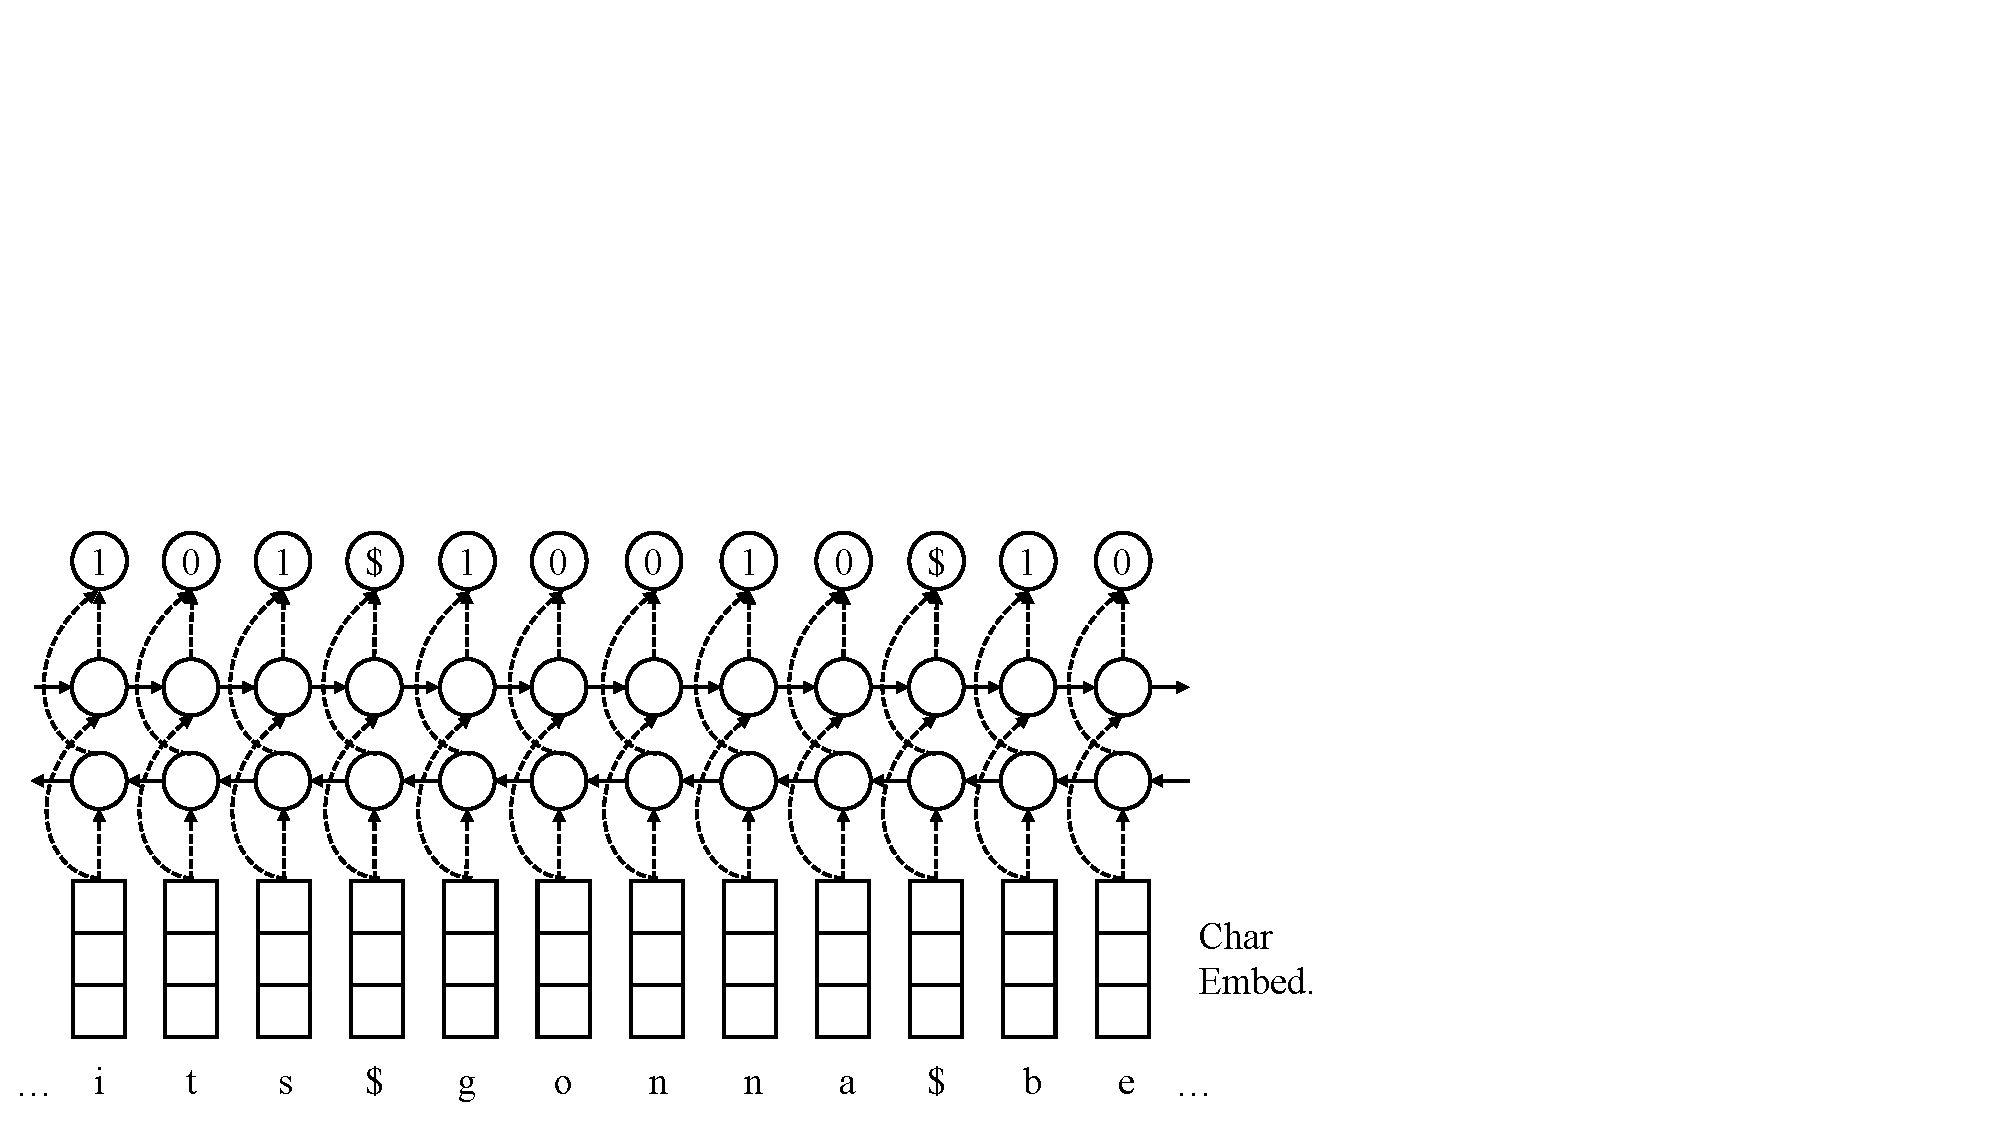
\includegraphics[width=\columnwidth,trim={0 0 11cm 9cm},clip]{graphics/bilstm_tokenizer}
	\caption{The bi-LSTM tokenizer that segments `{\it its gonna be}' into `{\it it s gon na be}'.}\label{fig:tok-model}
\end{figure}
We introduce a new
character-level bidirectional LSTM (bi-LSTM) sequence-labeling model
\cite{DBLP:journals/corr/HuangXY15,ma-hovy:2016:P16-1}
for tokenization.
Our model takes the raw sentence and tags each character in this 
sentence as whether it is the beginning of a word (1 as the beginning and 0 otherwise).
Figure \ref{fig:tok-model} shows the architecture of our tokenization model.
Space is treated as an input but deterministically  assigned a special tag \$.

\paragraph{Experimental results.}

\begin{table}[t]
	\centering
	\begin{tabular}{rc}
		\hline
		\it System & $F_1$ \\
		\hline
		  Stanford CoreNLP & 96.6 \\
		 Twokenizer & 94.4 \\		 
% 		UDPipe v1.2 & 94.7 \\
		\hdashline
		UDPipe v1.2 & 97.3 \\
	 	our bi-LSTM tokenizer & 98.3 \\
		\hline
	\end{tabular}
	\caption{Tokenizer comparison on the \textsc{Tweebank v2} test set.}\label{tbl:tok-result}
\end{table}
\citet{wang-EtAl:2017:Long6} show that the parser\nss{tokenizer?}\yjcomment{it's a parsing work.} trained 
on the combination of the UD\_English and Singapore English dialect (Singlish) treebanks
outperforms the one trained only on the dialect treebank.  Preliminary results
showed the same in our case, so 
we follow their work and trained our tokenizer on the training portion of
\textsc{Tweebank v2} combined with the UD\_English training set
and tested on the \textsc{Tweebank v2} test set. % \yicomment{should mention that combination of corpora improves the results, otherwise we should answer why we didn't try training ONLY on Tweebank v2}\yjcomment{add discussion}
We report $F_1$ scores, combining precision and recall for token identification. Table \ref{tbl:tok-result} shows the
tokenization results, compared to  other available tokenizers. 
 Stanford CoreNLP \cite{manning-EtAl:2014:P14-5} and Twokenizer
\cite{ICWSM101540} are rule-based systems and were not adapted
to the UD tokenization scheme.
The UDPipe v1.2
\cite{straka-strakova:2017:K17-3} model was re-trained on the same
data as our system. Compared with UDPipe, we use LSTM
instead of GRU in our model and we also use a larger size of hidden units (64 vs.~20),
which has stronger representation power. 
Our bi-LSTM tokenizer achieves the best accuracy among all these
tokenizers.  These results indicate the value of statistical modeling
in tokenization for informal texts.\nss{this paragraph needs copyediting}

\subsection{Part-of-Speech Tagger}

%\begin{figure}[t]
%	\centering
%	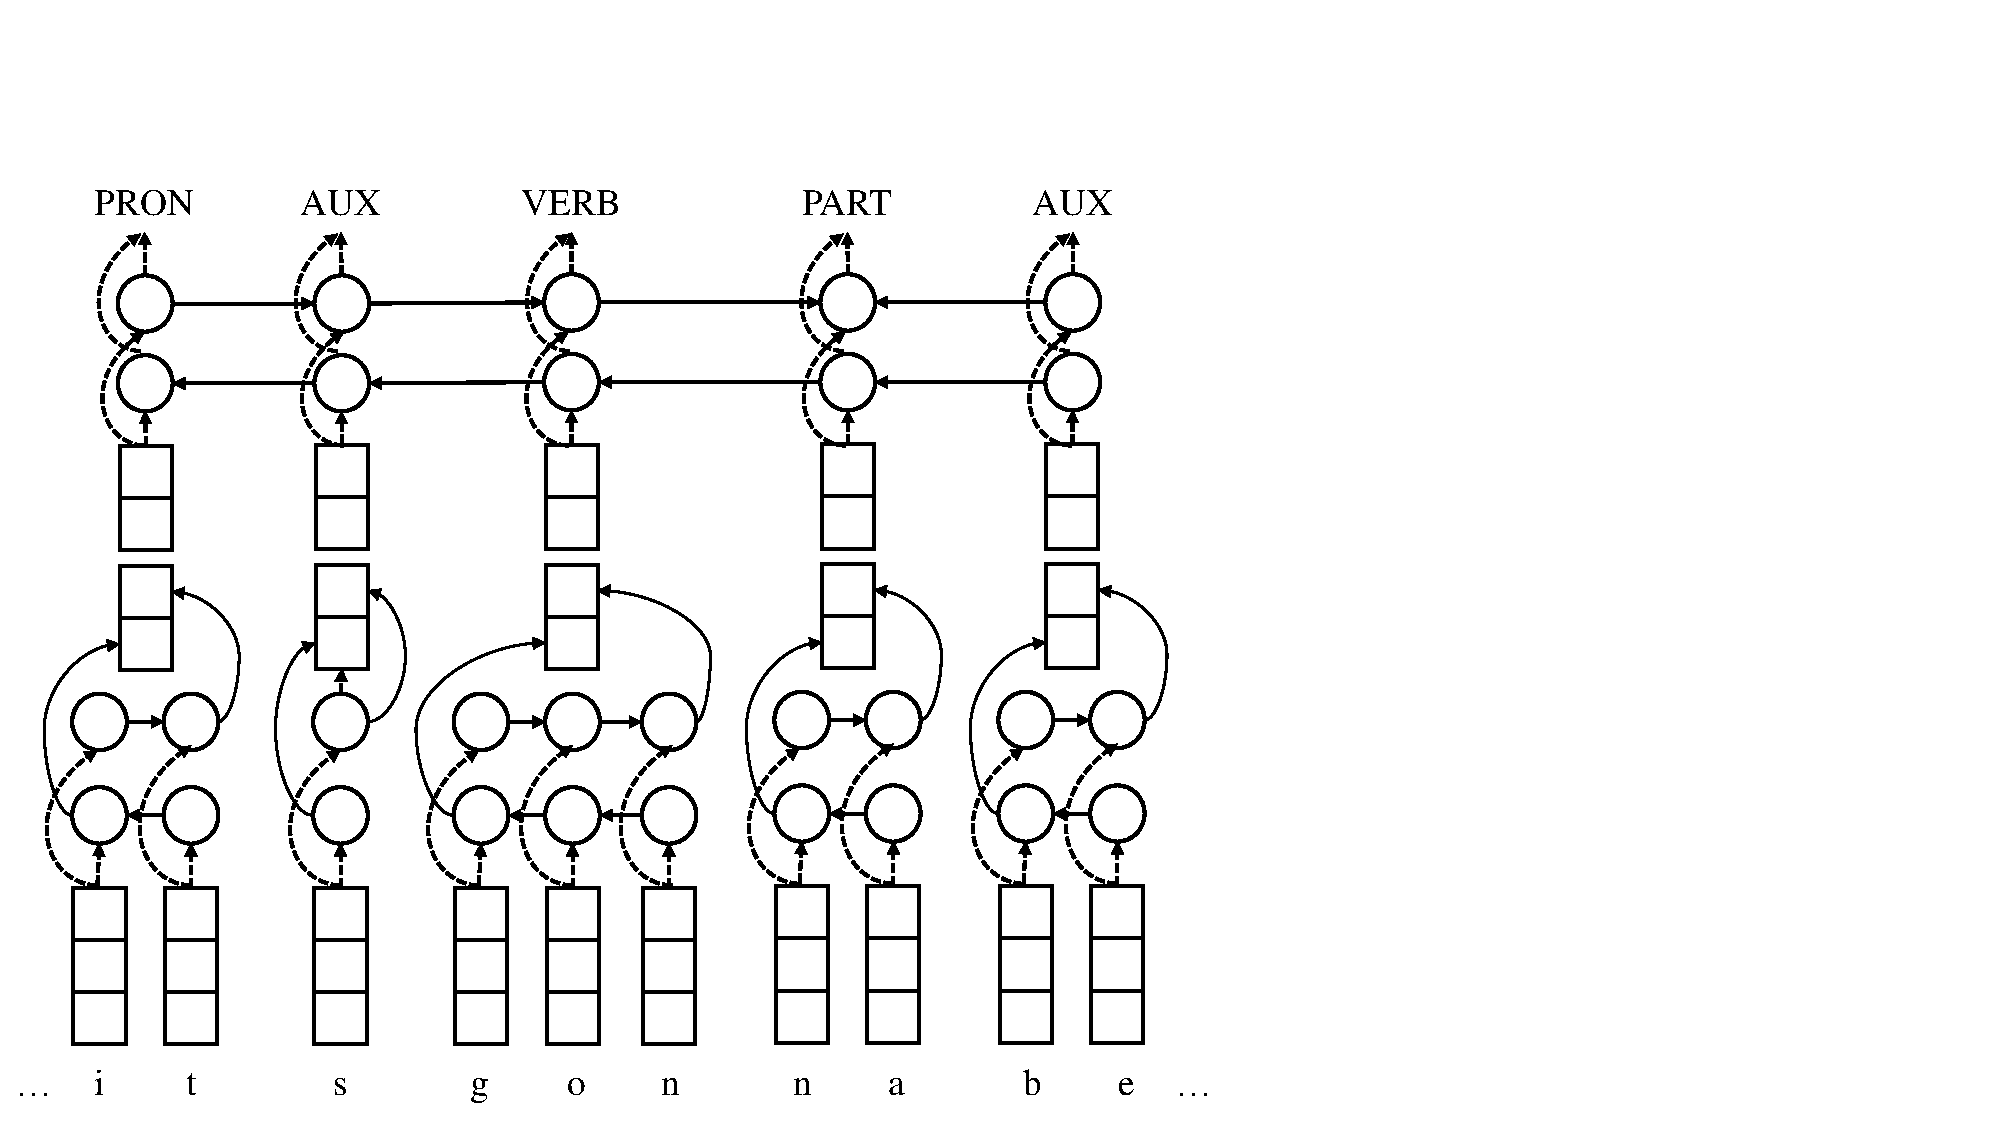
\includegraphics[width=\columnwidth,trim={0 0 11cm 3cm},clip]{graphics/bilstm_postagger}
%	\caption{The bi-LSTM POS tagger model that tags `it s gon na be' as {\tt PRON AUX VERB PART AUX}.}\label{fig:pos-model}
%	%\yicomment{i'm a little confused by the pic, need discussion}
%\end{figure}

Part-of-speech tagging for tweets has been extensively studied \cite{ritter-EtAl:2011:EMNLP,gimpel-EtAl:2011:ACL-HLT2011,derczynski-EtAl:2013:RANLP-2013,owoputi-EtAl:2013:NAACL-HLT,gui-EtAl:2017:EMNLP20172}. We therefore consider existing POS taggers for tweets instead of developing our own.
On the annotation scheme designed in \S\ref{sec:pos-anno}, based on UD and adapted for
Twitter, we compared several existing systems: the Stanford CoreNLP tagger, 
\citet{owoputi-EtAl:2013:NAACL-HLT}'s word cluster enhanced tagger
(both greedy and CRF variants), and 
\citet{ma-hovy:2016:P16-1}'s neural network tagger 
which achieves the state-of-the-art performance on PTB.
\citet{gui-EtAl:2017:EMNLP20172} presented a state-of-the-art neural tagger for Twitter,
but their implementation works only with the PTB tagset, so we exclude
it. % Thus, we didn't include their tagger in our comparison.\yjcomment{i put some words on \cite{gui-EtAl:2017:EMNLP20172} in case the reviewer challenge our neural/non-neural comparsion.}
 %and also two bi-LSTM systems similar
%to \citet{DBLP:journals/corr/HuangXY15} and \citet{lample-EtAl:2016:N16-1}, one using
%word vectors and the other using word and character vectors (see Figure \ref{fig:pos-model}).
All compared systems were re-trained on the combination of the UD\_English and 
\textsc{Tweebank v2} training sets. We use Twitter-specific GloVe embeddings released by
\citet{pennington-socher-manning:2014:EMNLP2014} in all neural taggers
and parsers.\footnote{\url{http://nlp.stanford.edu/data/glove.twitter.27B.zip}}


\paragraph{Experimental results.}

\begin{table}[t]
	\centering
	\begin{tabular}{rc}
		\hline
		\it System & Precision \\
		\hline
%		Stanford Postagger & 65.6 \\
		Stanford CoreNLP & 90.4 \\
%		UDPipe v1.2 & 78.7 \\
		\citealp{owoputi-EtAl:2013:NAACL-HLT} (greedy) & 94.2 \\
		\citealp{owoputi-EtAl:2013:NAACL-HLT} (CRF) & 95.1 \\
		\hdashline
%		UDPipe v1.2 & 83.8 \\
		\citealp{ma-hovy:2016:P16-1} & 91.8 \\
%		our word bi-LSTM & 89.2 \\
%		our character + word bi-LSTMs & 91.5 \\
		\hline
	\end{tabular}
	\caption{POS tagger comparison on gold-standard tokens in the
          \textsc{Tweebank v2} test set. \label{tbl:pos-result}}
\end{table}

\begin{table}[t]
	\centering
	\begin{tabular}{rc}
		\hline
		\it Tokenization System & $F_1$ \\
		\hline
		Stanford CoreNLP & 92.1 \\
		our bi-LSTM tokenizer (\S\ref{sec:tok}) & 93.7 \\
		\hline
	\end{tabular}
	\caption{\citet{owoputi-EtAl:2013:NAACL-HLT} POS tagging performance with automatic tokenization on
          the \textsc{Tweebank v2} test set. \label{tbl:pos-result-vs-tok}}
\end{table}

We tested the POS taggers on the \textsc{Tweebank v2} test set.  Results
with gold-standard tokenization are shown in
Table \ref{tbl:pos-result}. The careful feature engineering and making use of
\citet{Brown:1992:CNG:176313.176316} clusters in the 
POS tagger of \citet{owoputi-EtAl:2013:NAACL-HLT} outperforms \citet{ma-hovy:2016:P16-1}'s neural network
model. 
%tagger
%also makes use of clusters derived
%from a large collection of unannotated tweets. % Those clusters did not
%improve the performance of our bi-LSTM models.)

Results of the \citet{owoputi-EtAl:2013:NAACL-HLT}  tagger with non-greedy
inference on automatically tokenized data
are shown in  Table \ref{tbl:pos-result-vs-tok}.  We see that errors
in tokenization do propagate, but tagging performance is above 93\%
with our tokenizer. 

\subsection{Parser}

Social media applications typically require processing large volumes
of data, making speed an important consideration. We therefore 
begin with the neural greedy stack LSTM parser introduced by \newcite{ballesteros-EtAl:2016:EMNLP2016},
which can parse a sentence in linear time and harnesses 
character representations to construct word vectors, which should help mitigate the challenge of
spelling variation. We encourage the reader to refer their paper for
more details about the model.

In our preliminary experiments, we train our parser on the combination of UD\_English
and \textsc{Tweebank v2} training sets. Gold-standard tokenization and automatic POS
tags are used. Automatic POS tags are assigned with 5-fold
jackknifing. Hyperparameters %, including the value of $\alpha$ in Equation \ref{eq:distill},
are tuned on the \textsc{Tweebank v2} development set. Unlabeled attachment score and
labeled attachment score (including punctuation) are reported.
All the experiments were run on a Xeon E5-2670 2.6 GHz machine.

\citet{reimers-gurevych:2017:EMNLP2017} and others have
pointed out that neural network training is 
nondeterministic and depends on the seed for the random
number generator.
Our preliminary experiments confirm this finding, with a gap of 1 LAS on development data
between the best (75.8)
 and worst (74.8) runs. To control for this
effect, we report the average of five differently-seeded runs, for
each of our models and the compared ones.

\begin{table}[t]
	\centering
	\begin{tabular}{rccc}
		\hline
		\it System & UAS & LAS & Kt/s \\
		\hline
		\citet{kong-EtAl:2014:EMNLP2014} &81.6 & 77.2 & 0.3 \\
		\citet{dozat-qi-manning:2017:K17-3} & 81.9 &  77.7 & 1.7 \\
%		\newcite{dyer-EtAl:2015:ACL-IJCNLP} & 77.9 & 73.0 \\
		\newcite{ballesteros-EtAl:2016:EMNLP2016} & 80.4 & 75.8 & 2.3 \\
		\hdashline
		Ensemble (20) & 83.5 & 79.4 & 0.2 \\
		Distillation ($\alpha =1.0$) & 82.2 & 78.0 & 2.3 \\
		Distillation ($\alpha =0.9$) & 82.4 & 78.1 & 2.3 \\		
		Distillation w/ exploration & 82.5 & 78.4 & 2.3 \\
		\hline
	\end{tabular}
	\caption{Dependency parser comparison on \textsc{Tweebank v2} test set,
           with automatic POS tags. The ``Kt/s'' column shows
           the parsing speed evaluated by thousands of tokens
           the model processed per second.
            \label{tbl:parse-result}}
\end{table}

\paragraph{Initial results.}  The first section of Table~\ref{tbl:parse-result} compares
the stack LSTM with {\sc TweeboParser} (the system 
of \citealp{kong-EtAl:2014:EMNLP2014}) and the state-of-the-art parser
in the CoNLL 2017 evaluations, due to
 \citet{dozat-qi-manning:2017:K17-3}.
 \citet{kong-EtAl:2014:EMNLP2014}'s parser is a graph-based
parser with lexical features and word cluster and it uses dual decomposition
for decoding. The parser in \citet{dozat-qi-manning:2017:K17-3} is also a graph-based parser
but includes character-based word representation and uses the biaffine classifier
to predict if an attachment exists between two words.
Both of the compared systems require superlinear runtime due to graph-based parsing. 
They are re-trained on the same data as our
system.
Our baseline lags behind by nearly two LAS
points but runs faster than both of them.

\paragraph{Ensemble.}  Due to ambiguity in the training
data---which most loss functions are not robust to \citep{Frnay2014ClassificationIT}, including the log loss we use, following
\citet{ballesteros-dyer-smith:2015:EMNLP}---and due to the instability
of neural network training, we follow \citet{Dietterich2000} and
consider an ensemble of twenty parsers trained using different random
initialization.  To parse at test time, the transition probabilities of the twenty
members of the ensemble are averaged.  The result achieves LAS of
79.4, outperforming all three systems above (Table~\ref{tbl:parse-result}).

\paragraph{Distillation.}  The shortcoming of the 20-parser ensemble is, of
course, that it requires twenty times the runtime of a single greedy
parser, making it the slowest system in our comparison.  \newcite{kuncoro-16} proposed the distillation of 20
greedy transition-based parser into a single \emph{graph-based}
parser; they transformed the votes of the ensemble into a structured
loss function.  However, as Kuncoro et al.~pointed out, 
it is not straightforward to use a structured
loss in a \emph{transition-based} parsing algorithm.  Because fast
runtime is so important for NLP on social media, we
introduce a new way to distill our greedy ensemble into a single
transition-based parser (the first such attempt, to our knowledge).  

Our approach applies techniques from \newcite{DBLP:journals/corr/HintonVD15}
and \newcite{kim-rush:2016:EMNLP2016} to parsing.
Note that training a transition-based parser typically involves the
transformation of the training data into a sequence of ``oracle'' state-action
pairs.
Let $q(a \mid s)$ denote the distilled model's
probability of an action $a$ given parser state $s$; let $p(a\mid s)$ be the probability under the
ensemble (i.e., the average of the 20 separately-trained ensemble
members).
To train the distilled model, we minimize the interpolation between
their distillation loss and the conventional log loss:
\begin{align}
{\argmin}_q \quad  & \alpha \sum_i \underbrace{\sum_{a} -p(a
	\mid s_i) \cdot \log q(a \mid s_i)}_{\text{distillation loss}} \\
& +\ (1 - \alpha) \sum_i \underbrace{- \log q(a_i \mid
  s_i)}_{\text{log loss}} \nonumber
\end{align}

Distilling from this 
parser leads to a single greedy transition-based parser with 78.1
LAS---better than past systems but worse than our more expensive ensemble.
The effect of $\alpha$ is illustrated in
Figure~\ref{fig:effect-alpha}; generally paying closer attention to
the ensemble, rather than the conventional log loss objective, leads
to better performance.

\begin{figure}[t]
	\centering
	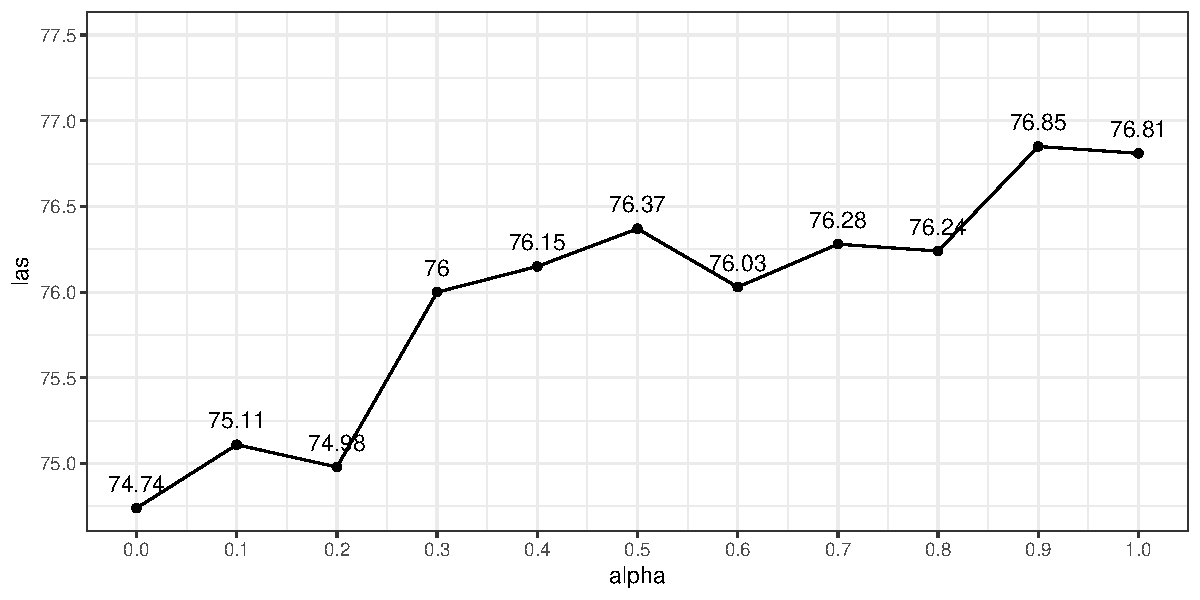
\includegraphics[width=\columnwidth,trim={0.3cm 0 0 0},clip]{graphics/alpha}
	\caption{The effect of $\alpha$ on distillation. \label{fig:effect-alpha}}
\end{figure}

\paragraph{Learning from exploration.} When we set $\alpha =1$, we
eliminate the oracle from the estimation procedure (for the distilled
model).  This presents an opportunity to learn with \emph{exploration}, by
randomly sampling transitions from the ensemble, found useful
in recent methods for training greedy models that use dynamic oracles
\citet{goldberg-nivre:2012:PAPERS,TACL145,TACL885,ballesteros-EtAl:2016:EMNLP2016}.  
We find that this
approach outperforms the  conventional distillation model, coming in
only one point behind the ensemble (last line of Table~\ref{tbl:parse-result}).

%
%\begin{table}[t]
%	\centering
%	\begin{tabular}{rcc}
%		\hline
%		\it System & UAS & LAS \\
%		\hline
%		\newcite{kuncoro-16} & 94.3 & 92.1 \\
%		\citet{DBLP:journals/corr/DozatM16} & 95.7 & 94.1 \\
%		\hdashline
%		\newcite{dyer-EtAl:2015:ACL-IJCNLP} & 93.0 & 90.9 \\		
%		%		\newcite{dyer-EtAl:2015:ACL-IJCNLP} & 77.9 & 73.0 \\
%		Ensemble (20) & 94.5 & 92.6 \\
%		Distillation ($\alpha =1.0$) & 93.8 & 91.7 \\
%		Distillation with exploration  & 94.1 & 92.0 \\
%		\hline
%	\end{tabular}
%	\caption{Dependency parser comparison on PTB test set.}\label{tbl:parse-result-PTB}
%\end{table}



%\nascomment{need to clarify:  is this UD?} We perform additional experiments on the Penn Treebank, following
%the settings of \newcite{dyer-EtAl:2015:ACL-IJCNLP};
%Table~\ref{tbl:parse-result-PTB} shows a similar trend, and we achieve
%performance close to that of the graph-based parser of \citet{kuncoro-16}.
%However, this greedy approach still lags behind the very strong
%graph-based system of \citet{DBLP:journals/corr/DozatM16}.

\begin{table}[t]
	\centering
	\begin{tabular}{rrcc}
		\hline
		\it Pipeline stage & Score & Ours & SOTA \\
		\hline
		Tokenization  & \it $F_1$ & 98.3 & 96.6 \\		
		POS tagging &  \it  $F_1$ & 93.7 & 92.1 \\
		UD parsing & \it LAS $F_1$ & 74.1 & 70.3 \\
		\hline
	\end{tabular}
	\caption{Evaluating our pipeline against a state-of-the-art pipeline. \label{tbl:pipline} %\yicomment{see tab5 for our tokenizer the pos tagging number is 93.6, here is 93.7, should be consistent}
	}
\end{table}

\paragraph{Pipeline evaluation.} Finally, we report  our full
pipeline's performance in  Table \ref{tbl:pipline}. We also compare
our model with a pipeline of the state-of-the-art systems (labeled  ``SOTA''):
Stanford CoreNLP tokenizer\footnote{We choose Stanford CoreNLP tokenizer in the spirit of comparing rule-based and statistical model-based method.}, %\yicomment{why not compare with UDPipe?}\yjcomment{i was thinking stanford tokenizer is more suitable, but i will get the udpipe result},
\citet{owoputi-EtAl:2013:NAACL-HLT}'s tagger, and \citet{dozat-qi-manning:2017:K17-3}'s parser.
Our system differs from the SOTA pipeline in the tokenization and parser components.
From Table \ref{tbl:pipline}, our pipeline outperforms the SOTA when
evaluated in pipeline manner.
The results also emphasize the
importance of tokenization:  without gold tokenization
%\nascomment{changed ``segmentation'' to ``tokenization'' here, twice},
UD parsing
performance drops by more than four points.

%\section{Related Work}
%\yjcomment{related word is not finished.}
%\newcite{eisenstein:2013:NAACL-HLT} reviewed NLP approaches for analyzing text on social media, especially for tweets and showed that there are two major directions for NLP community to handle the tweets, including normalization and domain adaptation. He also pointed out that normalization can be problematic because precisely defining the normalization task is difficult. 
%
%\newcite{kong-EtAl:2014:EMNLP2014} argues that the Penn Treebank approach to annotation is poorly suited to more informal genres of text, as some of the annotation challenges for tweets,
%including token selection, multiword expressions, multiple roots, and structure within noun phrases diverge significantly from conventional approaches. 
%They believe that rapid, small scale annotation efforts performed by imperfectly-trained annotators should provide enough evidence to train an effective parser, given the rapidly changing nature of tweets~\cite{eisenstein:2013:NAACL-HLT}, the attested difficulties of domain adaptation for parsing~\cite{dred07}, and the expense of creating Penn Treebank-style annotations~\cite{penn93}. 
%Therefore, they build a new corpus of tweets (Tweebank), with conventions informed by the domain, using new syntactic annotations that can tackle all the forementioned problems annotated in a day by two dozen annotators, most of whom had only cursory training in the annotation scheme. Then, they modify the decoder of the TurboParser, a graph-based dependency parser, which is open-source and has been found to perform well on a range of parsing problems in different languages~\cite{turbo13} to adapt to the Tweebank dataset, and incorporate new features such as Brown Clusters and Penn Treebank features and changes to specification
%in the output space into TurboParser.
%
%Like ``mfw'' is usually followed by an adverbial clause and ``ima'' is usually followed by a clausal complement. 
%It is not reasonable to treat them in the same part-of-speech. 
%In this paper, when annotating the POS tagging for abbreviations, we first try to recover their original forms, then use the POS of the core-word as the POS for the abbreviation.
%Second, four special POS tags (S, L, M, Y) were designed to handle contraction words in Gimpel et al. \shortcite{Gimpel:2011:PTT:2002736.2002747}. Major concern of designing such tags is to minimize the effort of tokenization. 
%However, contractions of common nouns and pronouns are casted into the same category which increase the difficulty of distinguishing their syntactic function (say, there's and book'll are treated with the same syntactic function). What's more, only a small proportion of words can be categorized into these tags (2.7 \% in total), which cast a doubt of the usefulness of these certain tags. In this paper, we believe such contraction can be properly handled by tokenization module, so we suggest to tokenize the contraction word and annotate POS tag accordingly.
%Besides the contraction that be conventionally tokenized, tweets also witness a set of unconventional contraction like iv (I've), whatis (what is). In this paper, we follow the same idea of annotation abbreviation to handle the unconventional contractions and use the POS of core word of the original form as their POS.
%Third, special POS was designed to handle emoticon in Gimpel et al. \shortcite{Gimpel:2011:PTT:2002736.2002747}. However, in most cases, emoticon plays the same role as most of the symbolic tokens. In this paper, we follow the UD guideline to annotate the emoticon as symbol (SYM).
%At last, it’s arguable that some of the hashtags, URLs can work as a nominal in tweets. Whether treating them as the same part-of-speech or different ones according to their context is an open question. A preliminary survey on the standard UD English data shows that URL, email address are all tagged as the foreign language (X), so we also tag them as X and leave the disambiguation of their syntactic function to the annotation of parse tree.

\section{Conclusion}
We study the problem of parsing tweets into Universal Dependencies.
We adapt the UD guidelines to cover 
special constructions in tweets and create
the {\sc Tweebank v2}, which has 55,607 tokens. We characterize the disagreements
among our annotators and argue that inherent ambiguity in this genre
makes
consistent annotation a challenge.  Using this new treebank,
we build a pipeline system to parse tweets into UD. We also 
propose a new method to distill an ensemble of 20 greedy parsers into a single one
to overcome annotation noise without sacrificing efficiency.
Our parser achieves an improvement of 2.6  in LAS over a strong baseline
and outperforms other state-of-the-art parsers in both accuracy and speed.

\section*{Acknowledge}
We thank Elizabeth Clark, Lucy Lin, Nelson Liu, Kelvin Luu, Phoebe Mulcaire, 
Hao Peng, Maarten Sap, Chenhao Tan, Sam Thomson,
and the other colleagues in Georgetown University for the annotation efforts in the first round.
We also thank the anonymous  reviewers for their helpful comments and suggestions.
\yjcomment{fonding agency here and anyone else i miss.}
This work was supported by the National Key Basic Research
Program of China via grant 2014CB340503 and the
National Natural Science Foundation of China (NSFC) via
grant 61632011.

\bibliography{shortdb}
\bibliographystyle{acl_natbib}
\end{document}
